% CVPR 2022 Paper Template
% based on the CVPR template provided by Ming-Ming Cheng (https://github.com/MCG-NKU/CVPR_Template)
% modified and extended by Stefan Roth (stefan.roth@NOSPAMtu-darmstadt.de)

\documentclass[10pt,twocolumn,letterpaper]{article}

%%%%%%%%% PAPER TYPE  - PLEASE UPDATE FOR FINAL VERSION
%\usepackage[review]{cvpr}      % To produce the REVIEW version
%\usepackage{cvpr}              % To produce the CAMERA-READY version
\usepackage[pagenumbers]{cvpr} % To force page numbers, e.g. for an arXiv version

% Include other packages here, before hyperref.
\usepackage{graphicx}
\usepackage{amsmath}
\usepackage{amssymb}
\usepackage{gensymb}
\usepackage{booktabs}

% included packages
\usepackage{makecell}
\usepackage{colortbl}
\usepackage{xcolor}

% It is strongly recommended to use hyperref, especially for the review version.
% hyperref with option pagebackref eases the reviewers' job.
% Please disable hyperref *only* if you encounter grave issues, e.g. with the
% file validation for the camera-ready version.
%
% If you comment hyperref and then uncomment it, you should delete
% ReviewTempalte.aux before re-running LaTeX.
% (Or just hit 'q' on the first LaTeX run, let it finish, and you
%  should be clear).
\usepackage[pagebackref,breaklinks,colorlinks]{hyperref}


% Support for easy cross-referencing
\usepackage[capitalize]{cleveref}
\crefname{section}{Sec.}{Secs.}
\Crefname{section}{Section}{Sections}
\Crefname{table}{Table}{Tables}
\crefname{table}{Tab.}{Tabs.}

% For caption setup
\captionsetup[table]{aboveskip=3pt}
\captionsetup[table]{belowskip=2pt}
\captionsetup[figure]{aboveskip=5pt}
\captionsetup[figure]{belowskip=0pt}
\captionsetup{font=normal}

%%%%%%%%% PAPER ID  - PLEASE UPDATE
\def\cvprPaperID{*****} % *** Enter the CVPR Paper ID here
\def\confName{CVPR}
\def\confYear{2022}


% utils
\newcommand{\correct}[1]{\textcolor{blue}{#1 \checkmark}}
\newcommand{\wrong}[1]{\textcolor{red}{#1 $\times$}}

\begin{document}

%%%%%%%%% TITLE - PLEASE UPDATE
\title{Tips for Writing a Research Paper using \LaTeX}

\author{Guanying Chen \\
{\tt\small \url{https://guanyingc.github.io}}
% For a paper whose authors are all at the same institution,
% omit the following lines up until the closing ``}''.
% Additional authors and addresses can be added with ``\and'',
% just like the second author.
% To save space, use either the email address or home page, not both
}
\onecolumn
\maketitle
{
    \hypersetup{linkcolor=black}
    \tableofcontents
}


%%%%%%%%% ABSTRACT

%%%%%%%%% BODY TEXT
%\newpage
\vspace{7em}

\section{Introduction}
\label{sec:intro}
\LaTeX\ is a very powerful tool for documentation preparation, and is often used by researchers to prepare a manuscript for reviewing and publication. 
However, some new graduate students might not have experience in using \LaTeX and thus have a difficult time in prepare their first paper. 

In this article, we will first provide some tips for paper writing.  
Then, we will showcase several working examples for the tables and figures, which have been used in our previous publications. The readers are encouraged to adapt those tables and figures to their purposes to save time when preparing their first papers.

\twocolumn

\section{Tips for the Writing}
In this section, we point out some common mistakes in paper writing and give some suggestions for editing \LaTeX\ files.

\subsection{Some Common Mistakes}
\begin{itemize}
    \item There should be a space before the open parentheses:\\
        \wrong{Convolutional neural network(CNN) has been successfully applied on various vision problems.}\\
        \correct{Convolutional neural network (CNN) has been successfully applied on various vision problems.}
    \item There should be no space before the period and comma punctuation marks:\\
        \wrong{Convolutional neural network (CNN) has been successfully applied on various vision problems .}\\
        \correct{Convolutional neural network (CNN) has been successfully applied on various vision problems.}
    \item There should be a punctuation at the end of the equation:
        \begin{align}
            \label{eq:eq1}
            & \textcolor{red}{E = mc^2 \quad \times} \\
            & \textcolor{blue}{E = mc^2. \quad \checkmark}
        \end{align}
    \item All equations should be numbered:
        \begin{align}
            \label{eq:eq2} \nonumber
            & \textcolor{red}{E = mc^2. \quad \times}\\ 
            & \textcolor{blue}{E = mc^2. \quad \checkmark}
        \end{align}
    \item The first character in a sentence should be capitalized:\\
        \wrong{how are you?}\\
        \correct{How are you?}
    \item Double quotation marks should be correctly typed:\\
        \wrong{Are you "okay"?}\\
        \correct{Are you ``okay''?}
    \item There should be a space before the citation:\\
        \wrong{A proposes a method B for this problem[1].}\\
        \correct{A proposes a method B for this problem~[1].}
\end{itemize}

\subsection{Some Suggestions}
\begin{itemize}
    \item Do not include citations in the abstract.
    \item Define a macro for a word or phrase if it appears frequently (\eg, the method name and the dataset name). The command can be\\``\textbackslash newcommand\{\textbackslash NetName\}\{A Great Deep Net\}''.
    \item Use ``\textbackslash ie'' command for ``\ie'' and use ``\textbackslash eg'' for ``\eg.''.
    \item When referring to a table, always use ``Table~\ref{tab:table1}'' in the sentence:\\
        \wrong{Our results are shown in Tab.~1.}\\
        \correct{Our results are shown in Table~1.}

    \item The table caption should be at the top of the table.
    \item When referring to a figure, use ``Figure~\ref{fig:figure1}'' at the beginning of a sentence and ``Fig.~\ref{fig:figure1}'' elsewhere.\\
        \wrong{Fig.1 shows our results.}\\
        \correct{Our results are shown in Fig.~1.}\\
        \correct{Figure~1 shows our results.}
    \item The figure caption should be at the bottom of the table.
    \item It is better to put the tables and figures at the top of a page.
\end{itemize}

\clearpage

\section{Examples for the Tables}

%\subsection{Examples for the Single-column Tables}
\begin{table}[thb]\centering
    \caption{A simple table with a header row.}
    \label{tab:table1}
    \resizebox{0.48\textwidth}{!}{
    \large
    \begin{tabular}{*{10}{c}}
        \toprule
       Data & Size &  2-Exp & 3-Exp &  4-Exp & 5-Exp &  6-Exp &  7-Exp \\
        \midrule
        A & $1280\times 720$ & 1 & 2 & 3 & 4 & 5 & 4 \\
        B & $1280\times 720$ & 1 & 2 & 3 & 4 & 5 & 4 \\
        Ours & $4096\times 2168$ & 2 & 3 & 4 & 6 & 5 & 4 \\
        \bottomrule
    \end{tabular}
    }
\end{table}
 % simple table
\begin{table}[thb]\centering
    \caption{A table with multi-column headers.}
    \label{tab:table2}
    \resizebox{0.48\textwidth}{!}{
    \large
    \begin{tabular}{*{10}{c}}
        \toprule
        &  &  \multicolumn{2}{c}{$6-9$ frames} & \multicolumn{2}{c}{$5-7$ frames} & \multicolumn{2}{c}{$50-200$ frames} \\
       Data & Size &  2-Exp & 3-Exp &  2-Exp & 3-Exp &  2-Exp & 3-Exp \\
        \midrule
        A & $1280\times 720$ & 1 & 2 & 3 & 4 & 5 & 4 \\
        B & $1280\times 720$ & 1 & 2 & 3 & 4 & 5 & 4 \\
        Ours & $4096\times 2168$ & 2 & 3 & 4 & 6 & 5 & 4 \\
        \bottomrule
    \end{tabular}
    }
\end{table}

 % multi-column table
% require package makecell 
\begin{table}[thb]\centering
    \caption{A table with line break in the header. Line break is useful if the item name is too long.}
    \label{tab:table3}
    \resizebox{0.48\textwidth}{!}{
    \large
    \begin{tabular}{*{10}{c}}
        \toprule
         %&  &  \multicolumn{3}{c}{\makecell{Static Scenes \\ w/ Ground Truth}} & \multicolumn{3}{c}{\makecell{Dynamic Scenes \\ w/o Ground Truth}} \\
        &  &  \multicolumn{3}{c}{$6-9$ frames} & \multicolumn{3}{c}{$5-7$ frames} \\
        Data & Size &  \makecell{2-Exp \\ Scenes} &  \makecell{2-Exp \\ Scenes} &  \makecell{2-Exp \\ Scenes} &  \makecell{2-Exp \\ Scenes} &  \makecell{2-Exp \\ Scenes} &  \makecell{2-Exp \\ Scenes} \\
        \midrule
        A & $1280\times 720$ & 1 & 2 & 3 & 4 & 5 & 4 \\
        B & $1280\times 720$ & 1 & 2 & 3 & 4 & 5 & 4 \\
        Ours & $4096\times 2168$ & 2 & 3 & 4 & 6 & 5 & 4 \\
        \bottomrule
    \end{tabular}
    }
\end{table}


 % multi-column with makecell
% require package makecell 
\begin{table}[thb]\centering
    \caption{A table with multi-column headers and vertical lines for grouping.}
    \label{tab:table4}
    \resizebox{0.48\textwidth}{!}{
    \large
    \begin{tabular}{c|c|ccc|ccc}
        \toprule
         %&  &  \multicolumn{3}{c}{\makecell{Static Scenes \\ w/ Ground Truth}} & \multicolumn{3}{c}{\makecell{Dynamic Scenes \\ w/o Ground Truth}} \\
        &  &  \multicolumn{3}{c|}{$6-9$ frames} & \multicolumn{3}{c}{$5-7$ frames} \\
        Data & Size &  \makecell{2-Exp \\ Scenes} &  \makecell{2-Exp \\ Scenes} &  \makecell{2-Exp \\ Scenes} &  \makecell{2-Exp \\ Scenes} &  \makecell{2-Exp \\ Scenes} &  \makecell{2-Exp \\ Scenes} \\
        \midrule
        A & $1280\times 720$ & 1 & 2 & 3 & 4 & 5 & 4 \\
        B & $1280\times 720$ & 1 & 2 & 3 & 4 & 5 & 4 \\
        Ours & $4096\times 2168$ & 2 & 3 & 4 & 6 & 5 & 4 \\
        \bottomrule
    \end{tabular}
    }
\end{table}


 % multi-column with vertical lines
% require package makecell 
\begin{table}[thb]\centering
    \caption{A table with multi-column headers and bold font highlights.}
    \label{tab:table5}
    \resizebox{0.48\textwidth}{!}{
    \large
    \begin{tabular}{c|c|ccc|ccc}
        \toprule
         %&  &  \multicolumn{3}{c}{\makecell{Static Scenes \\ w/ Ground Truth}} & \multicolumn{3}{c}{\makecell{Dynamic Scenes \\ w/o Ground Truth}} \\
        &  &  \multicolumn{3}{c|}{$6-9$ frames} & \multicolumn{3}{c}{$5-7$ frames} \\
        Data & Size &  \makecell{2-Exp \\ Break} &  \makecell{2-Exp \\ Break} &  \makecell{2-Exp \\ Break} &  \makecell{2-Exp \\ Break} &  \makecell{2-Exp \\ Break} &  \makecell{2-Exp \\ Break} \\
        \midrule
        A & $1280\times 720$ & 1 & 2 & 3 & 4 & \textbf{5} & \textbf{7} \\
        B & $1280\times 720$ & 1 & 2 & 3 & 4 & \textbf{5} & \textbf{7} \\
        Ours & $4096\times 2168$ & \textbf{2} & \textbf{3} & \textbf{4} & \textbf{6} & \textbf{5} & 4 \\
        \bottomrule
    \end{tabular}
    }
\end{table}


 % multi-column with bold font
% \usepackage{colortbl}  
% \usepackage{xcolor}

\begin{table}[thb]\centering
    \caption{A table with parallel lines for grouping and color highlight.} %
    \label{tab:ablation_study}
    \resizebox{0.48\textwidth}{!}{
    \Large
    \begin{tabular}{*{2}{l}||*{2}{c}||*{2}{c}||*{2}{c}}
        \toprule
        \multicolumn{1}{c}{} & \multicolumn{1}{c||}{} & \multicolumn{2}{c||}{Synthetic Dataset} & \multicolumn{2}{c||}{Static Data} & \multicolumn{2}{c}{Dynamicgt Data} \\
        ID & Method  & PSNRT & VDP & PSNRT & VDP & PSNRT & VDP \\
        \midrule
        0 & ANet  & 39.25 & 70.81 & 40.62 & 74.51 & 44.43 & 77.74 \\ %
        1 & BNet  & 39.69 & 70.95 & 37.61 & 75.30 & 43.70 & 78.97 \\
        \rowcolor{gray!20}
        2 & ANet + BNet  & \textbf{40.34} & \textbf{71.79} & \textbf{41.18} & \textbf{76.15} & \textbf{45.46} & \textbf{79.09} \\
        \midrule
        3 & ANet + BNet w/o C & 39.72 & 71.38 & 40.52 & 74.79 & 45.09 & 78.24 \\ %
        4 & ANet + BNet w/o D & 40.03 & 71.66 & 40.80 & 76.12 & 45.17 & 78.99 \\ %
        \bottomrule
    \end{tabular}
    }
\end{table}
 % multi-column with parallel lines
\begin{table}[h]
    \centering
    \caption{A table for illustrating the network architecture.}
    \label{tab:refineNet}
	\resizebox{0.48\textwidth}{!}{
        \small
        \begin{tabular}[t]{|*{6}{l|}}
        \hline
        \multicolumn{6}{|c|}{\textbf{RefineNet}} \\
        \hline
        \textbf{layer} & \textbf{k} & \textbf{s} & \textbf{chns} & \textbf{d-f} & \textbf{input} \\
        \hline 
        conv1   & 9     & 1    & 8/64   & 1    & Image+m\_1+a\_1+f\_1\\
        conv2   & 4     & 2    & 64/64  & 2    & conv1 \\
        conv3   & 4     & 2    & 64/64  & 4    & conv2 \\
        conv4   & 4     & 2    & 64/64  & 8    & conv3 \\
        \hline 
        ResBlock1 & 3     & 1  & 64/64  & 8    & conv4 \\
        ResBlock2 & 3     & 1  & 64/64  & 8    & ResBlock1 \\
        ResBlock3 & 3     & 1  & 64/64  & 8    & ResBlock2 \\
        ResBlock4 & 3     & 1  & 64/64  & 8    & ResBlock3 \\
        ResBlock5 & 3     & 1  & 64/64  & 8    & ResBlock4 \\
        \hline 
        deconv1\_a  & 4   & 2    & 64/64 & 4   & ResBlock5 \\
        deconv2\_a  & 4   & 2    & 64/64 & 2   & deconv1\_a \\
        deconv3\_a  & 4   & 2    & 64/64 & 1   & deconv2\_a \\
        \rowcolor{gray!25}
        a\_refined  & 3   & 1    & 65/1 & 1   & deconv3\_a+a\_1\\
        \hline
        deconv1\_f  & 4   & 2    & 64/64 & 4   & ResBlock5 \\
        deconv2\_f  & 4   & 2    & 64/64 & 2   & deconv1\_f \\
        deconv3\_f  & 4   & 2    & 64/64 & 1   & deconv2\_f \\
        \rowcolor{gray!25}
        f\_refined        & 3   & 1    & 66/2 & 1   & deconv3\_f+f\_1\\
        \hline
        \end{tabular}
    }
\end{table}
 % single-column network arch

\begin{table}[thb] \centering
    \caption{A table with images at the left. Images can be useful to illustrate different setups.} 
    \label{tab:res_synth_mirco_baseline}
    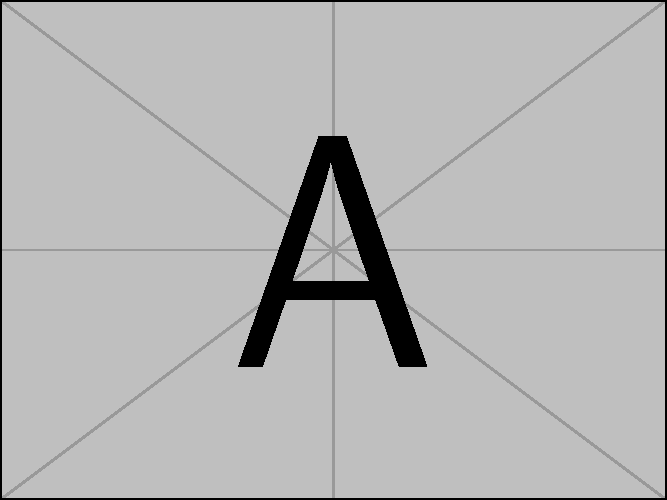
\includegraphics[width=0.088\textwidth,height=0.085\textwidth]{example-image-a}
    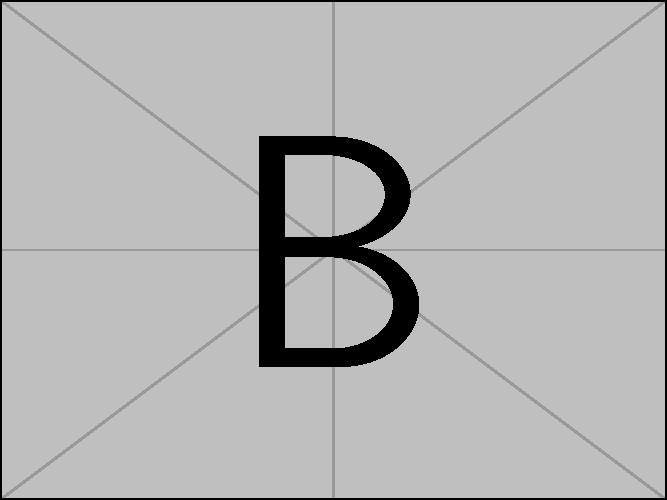
\includegraphics[width=0.088\textwidth,height=0.085\textwidth]{example-image-b}
    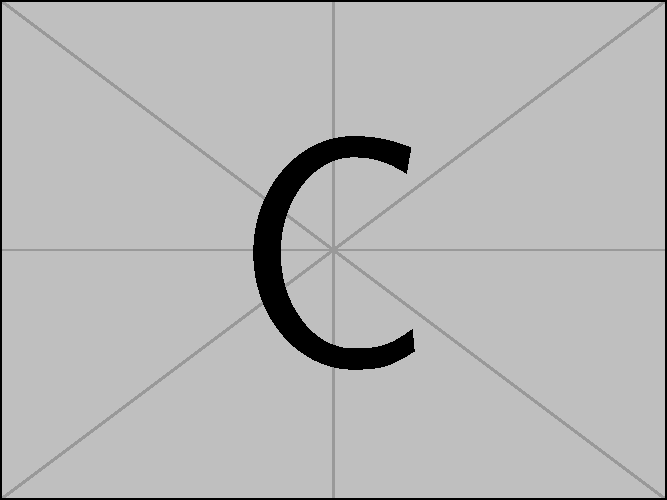
\includegraphics[width=0.088\textwidth,height=0.085\textwidth]{example-image-c}
    \raisebox{0.9\height}{
    \resizebox{0.19\textwidth}{!}{
    \large
    \begin{tabular}{ccc}
        \toprule
        Type & Range & MAE \\
        \midrule
        (a) & 144$\times$144 & 4.21 \\ 
        (b) & 37$\times$37 & 10.90 \\
        (c) & 22$\times$22 & 18.72 \\
        \bottomrule
    \end{tabular}
    }}
    \\
    \vspace{-0.2em}
    \makebox[0.09\textwidth]{\footnotesize (a)} 
    \makebox[0.09\textwidth]{\footnotesize (b)}
    \makebox[0.09\textwidth]{\footnotesize (c)}
    \makebox[0.19\textwidth]{\footnotesize (d) Normal estimation}
    \\
\end{table}
 % table with images

%\subsection{Examples for the Two-column Tables}
\begin{table*}[thb] \centering
    \caption{A two-column table.}
    \label{tab:table8}
    \resizebox{\textwidth}{!}{
    \Huge
        \begin{tabular}{c|*{4}{c}|*{4}{c}|*{4}{c}|*{4}{c}|*{4}{c}}
        \toprule
        & \multicolumn{4}{c}{Glass} 
                               & \multicolumn{4}{c}{Object A} 
                               & \multicolumn{4}{c}{Object B} 
                               & \multicolumn{4}{c}{Object C}  
                               & \multicolumn{4}{c}{Average}  \\
                               & F-EPE & A-MSE & I-MSE &  M-IoU 
                               & F-EPE & A-MSE & I-MSE &  M-IoU 
                               & F-EPE & A-MSE & I-MSE &  M-IoU 
                               & F-EPE & A-MSE & I-MSE &  M-IoU 
                               & F-EPE & A-MSE & I-MSE &  M-IoU \\
        \midrule
        Method A    & 3.6 / 30.3 & 1.33 & 0.48 & 0.12 & 6.4 / 53.2 & 1.54 & 0.68 & 0.12 & 10.3 / 39.2 & 1.94 & 1.57 & 0.24 & 6.8 / 56.8 & 2.50 & 0.85 & 0.11 & 6.8 / 44.9 & 1.83 & 0.90 & 0.15 \\
        Method B     & 2.1 / 15.8 & 0.22 & 0.14 & 0.97 & 3.1 / 23.5 & 0.31 & 0.23 & 0.97 & 2.0 / 6.7   & 0.17 & 0.28 & 0.99 & 4.5 / 34.4 & 0.38 & 0.33 & 0.92 & 2.9 / 20.1 & 0.27 & 0.24 & 0.96 \\
        \midrule
        Method C       & 1.9 / 14.7 & 0.21 & 0.14 & 0.97 & 2.9 / 21.8 & 0.30 & 0.22 & 0.97 & 1.9 / 6.6   & 0.15 & 0.29 & 0.99 & 4.1 / 31.5 & 0.37 & 0.32 & 0.92 & 2.7 / 18.6 & 0.26 & 0.24 & 0.96 \\
        \bottomrule
    \end{tabular}
    }
\end{table*}
 % two-column table
\begin{table*} \centering
    \caption{A two-column table with remark.}
    \label{tab:table8}
    \resizebox{\textwidth}{!}{
    \Huge
        \begin{tabular}{c|*{4}{c}|*{4}{c}|*{4}{c}|*{4}{c}|*{4}{c}}
        \toprule
        & \multicolumn{4}{c}{Glass} 
                               & \multicolumn{4}{c}{Object A} 
                               & \multicolumn{4}{c}{Object B} 
                               & \multicolumn{4}{c}{Object C}  
                               & \multicolumn{4}{c}{Average}  \\
                               & F-EPE & A-MSE & I-MSE &  M-IoU 
                               & F-EPE & A-MSE & I-MSE &  M-IoU 
                               & F-EPE & A-MSE & I-MSE &  M-IoU 
                               & F-EPE & A-MSE & I-MSE &  M-IoU 
                               & F-EPE & A-MSE & I-MSE &  M-IoU \\
        \midrule
        Method A    & 3.6 / 30.3 & 1.33 & 0.48 & 0.12 & 6.4 / 53.2 & 1.54 & 0.68 & 0.12 & 10.3 / 39.2 & 1.94 & 1.57 & 0.24 & 6.8 / 56.8 & 2.50 & 0.85 & 0.11 & 6.8 / 44.9 & 1.83 & 0.90 & 0.15 \\
        Method B$^*$     & 2.1 / 15.8 & 0.22 & 0.14 & 0.97 & 3.1 / 23.5 & 0.31 & 0.23 & 0.97 & 2.0 / 6.7   & 0.17 & 0.28 & 0.99 & 4.5 / 34.4 & 0.38 & 0.33 & 0.92 & 2.9 / 20.1 & 0.27 & 0.24 & 0.96 \\
        \midrule
        Method C       & 1.9 / 14.7 & 0.21 & 0.14 & 0.97 & 2.9 / 21.8 & 0.30 & 0.22 & 0.97 & 1.9 / 6.6   & 0.15 & 0.29 & 0.99 & 4.1 / 31.5 & 0.37 & 0.32 & 0.92 & 2.7 / 18.6 & 0.26 & 0.24 & 0.96 \\
        \bottomrule
    \end{tabular}
    }
    \vspace{-1em}
    \begin{flushleft}
        \footnotesize ${^*}$ indicates that method B is trained from scratch.
    \end{flushleft}
\end{table*}
 % two-column table with remarks
\begin{table*} \centering
    \caption{A two-column table with color header.}
    \label{tab:table9}
    \begin{minipage}{0.93\textwidth}
    \resizebox{\textwidth}{!}{
    \Huge
        \begin{tabular}{c|*{4}{c}|*{4}{c}|*{4}{c}|*{4}{c}|*{4}{c}}
        \toprule
        & \multicolumn{4}{c}{Glass} 
                               & \multicolumn{4}{c}{Glass with Water} 
                               & \multicolumn{4}{c}{Lens} 
                               & \multicolumn{4}{c}{Complex Shape}  
                               & \multicolumn{4}{c}{Average}  \\
                               & \cellcolor{red!25} F-EPE & \cellcolor{red!25}A-MSE & \cellcolor{red!25}I-MSE & \cellcolor{blue!25} M-IoU 
                               & \cellcolor{red!25} F-EPE & \cellcolor{red!25}A-MSE & \cellcolor{red!25}I-MSE & \cellcolor{blue!25} M-IoU 
                               & \cellcolor{red!25} F-EPE & \cellcolor{red!25}A-MSE & \cellcolor{red!25}I-MSE & \cellcolor{blue!25} M-IoU 
                               & \cellcolor{red!25} F-EPE & \cellcolor{red!25}A-MSE & \cellcolor{red!25}I-MSE & \cellcolor{blue!25} M-IoU 
                               & \cellcolor{red!25} F-EPE & \cellcolor{red!25}A-MSE & \cellcolor{red!25}I-MSE & \cellcolor{blue!25} M-IoU \\
        \midrule
        Method A    & 3.6 / 30.3 & 1.33 & 0.48 & 0.12 & 6.4 / 53.2 & 1.54 & 0.68 & 0.12 & 10.3 / 39.2 & 1.94 & 1.57 & 0.24 & 6.8 / 56.8 & 2.50 & 0.85 & 0.11 & 6.8 / 44.9 & 1.83 & 0.90 & 0.15 \\
        Method B     & 2.1 / 15.8 & 0.22 & 0.14 & 0.97 & 3.1 / 23.5 & 0.31 & 0.23 & 0.97 & 2.0 / 6.7   & 0.17 & 0.28 & 0.99 & 4.5 / 34.4 & 0.38 & 0.33 & 0.92 & 2.9 / 20.1 & 0.27 & 0.24 & 0.96 \\
        \midrule
        Method C       & 1.9 / 14.7 & 0.21 & 0.14 & 0.97 & 2.9 / 21.8 & 0.30 & 0.22 & 0.97 & 1.9 / 6.6   & 0.15 & 0.29 & 0.99 & 4.1 / 31.5 & 0.37 & 0.32 & 0.92 & 2.7 / 18.6 & 0.26 & 0.24 & 0.96 \\
        \bottomrule
    \end{tabular}
    }
    \end{minipage}
    \hspace{-0.6em}
    \begin{minipage}{0.06\textwidth}
        \resizebox{\textwidth}{!}{
        \begin{tabular}{cc}
            \midrule
            MSE ($\cdot10^{-2}$) \\
            \cellcolor{red!25} $\downarrow$ better \\ 
            \cellcolor{blue!25} $\uparrow$ better\\
            \midrule
        \end{tabular}
        }
    \end{minipage}
\end{table*}

 % two-column table with color header
\newcommand{\PSNRT}{PSNR\xspace}
\newcommand{\VQM}{HDR-VQM\xspace}
\newcommand{\VDP}{HDR-VDP2\xspace}
\newcommand{\LowExposure}{Low-Exposure\xspace}
\newcommand{\MiddleExposure}{Middle-Exposure\xspace}
\newcommand{\HighExposure}{High-Exposure\xspace}
\newcommand{\AllExposure}{All-Exposure\xspace}

\newcommand{\Frst}[1]{\textcolor{red}{\textbf{#1}}}
\newcommand{\Scnd}[1]{\textcolor{blue}{\textbf{#1}}}

\begin{table*}[t] \centering
    \caption{A two-column table with two sub-tables. \Frst{Red} text indicates the best and \Scnd{blue} text indicates the second best result, respectively.}
    \label{tab:res_real_data_wide}
    \makebox[\textwidth]{\small (a) Results on dataset A.} 
    \resizebox{\textwidth}{!}{
        \Large
    \begin{tabular}{l||*{2}{c}|*{2}{c}|*{3}{c}||*{2}{c}|*{2}{c}|*{2}{c}|*{3}{c}}
        \toprule
        & \multicolumn{7}{c||}{2-Exposure} & \multicolumn{9}{c}{3-Exposure} \\
        & \multicolumn{2}{c}{\LowExposure} & \multicolumn{2}{c}{\HighExposure} & \multicolumn{3}{c||}{\AllExposure} & \multicolumn{2}{c}{\LowExposure} & \multicolumn{2}{c}{\MiddleExposure} & \multicolumn{2}{c}{\HighExposure} & \multicolumn{3}{c}{\AllExposure} \\
        Method & \PSNRT & \VDP & \PSNRT & \VDP  & \PSNRT & \VDP & \VQM & \PSNRT & \VDP & \PSNRT & \VDP  & \PSNRT & \VDP & \PSNRT & \VDP & \VQM \\
        \midrule
        Method A & \Scnd{40.00} & 73.70 & \Scnd{40.04} & \Scnd{70.08} & \Scnd{40.02} & 71.89 & \Scnd{76.22} 
                      & \Scnd{39.61} & 73.24 & \Frst{39.67} & \Frst{73.24} & \Frst{40.01} & 67.90 & \Frst{39.77} & 70.37 & 79.55 \\
        Method B      & 34.54 & 80.22 & 39.25 & 65.96 & 36.90 & 73.09 & 65.33 
                      & 36.51 & 77.78 & 37.45 & 69.79 & 39.02 & 64.57 & 37.66 & 70.71 & 70.13 \\
        Method C  & 39.79 & \Scnd{81.02} & 39.96 & 67.25 & 39.88 & \Scnd{74.13} & 73.84 
                      & 39.48 & \Scnd{78.13} & 38.43 & 70.08 & 39.60 & \Scnd{67.94} & 39.17 & \Scnd{72.05} & \Scnd{80.70} \\
        Ours          & \Frst{41.95} & \Frst{81.03} & \Frst{40.41} & \Frst{71.27} & \Frst{41.18} & \Frst{76.15} & \Frst{78.84}
                      & \Frst{40.00} & \Frst{78.66} & \Scnd{39.27} & \Scnd{73.10} & \Scnd{39.99} & \Frst{69.99} & \Scnd{39.75} & \Frst{73.92} & \Frst{82.87} \\
        \bottomrule
    \end{tabular}
    }

    \vspace{0.5em}
    \makebox[\textwidth]{\small (b) Results on dataset B.} 
    \resizebox{\textwidth}{!}{
        \Large
    \begin{tabular}{l||*{2}{c}|*{2}{c}|*{3}{c}||*{2}{c}|*{2}{c}|*{2}{c}|*{3}{c}}
        \toprule
        & \multicolumn{7}{c||}{2-Exposure} & \multicolumn{9}{c}{3-Exposure} \\
        & \multicolumn{2}{c}{\LowExposure} & \multicolumn{2}{c}{\HighExposure} & \multicolumn{3}{c||}{\AllExposure} & \multicolumn{2}{c}{\LowExposure} & \multicolumn{2}{c}{\MiddleExposure} & \multicolumn{2}{c}{\HighExposure} & \multicolumn{3}{c}{\AllExposure} \\
        Method & \PSNRT & \VDP & \PSNRT & \VDP  & \PSNRT & \VDP & \VQM & \PSNRT & \VDP & \PSNRT & \VDP  & \PSNRT & \VDP & \PSNRT & \VDP & \VQM \\
        \midrule
        Method A & 37.73 & 74.05 & 45.71 & 66.67 & 41.72 & 70.36 & 85.33 
                      & 37.53 & 72.03 & 36.38 & 65.37 & 34.73 & 62.24 & 36.21 & 66.55 & 84.43 \\
        Method B      & 36.41 & 85.68 & \Scnd{49.89} & \Scnd{69.90} & 43.15 & 77.79 & 78.92 
                      & 36.43 & 77.74 & 39.80 & \Scnd{67.88} & \Scnd{43.03} & \Scnd{64.74} & 39.75 & \Scnd{70.12} & 87.93 \\
        Method C  & \Scnd{39.94} & \Scnd{86.77} & 49.49 & 69.04 & \Scnd{44.72} & \Scnd{77.91} & \Scnd{87.16} 
                      & \Scnd{38.34} & \Scnd{78.04} & \Scnd{41.21} & 66.07 & 42.66 & 64.01 & \Scnd{40.74} & 69.37 & \Scnd{89.36}\\
        Ours          & \Frst{40.83} & \Frst{86.84} & \Frst{50.10} & \Frst{71.33} & \Frst{45.46} & \Frst{79.09} & \Frst{87.40} 
                      & \Frst{38.77} & \Frst{78.11} & \Frst{41.47} & \Frst{68.49} & \Frst{43.24} & \Frst{65.08} & \Frst{41.16} & \Frst{70.56} & \Frst{89.56}\\
        \bottomrule
    \end{tabular}
    }
\end{table*}
 % two-column table with two sub-tables
\begin{table*}[t]
\centering
    \caption{A two-column table with \textbackslash cmidrule for grouping without using vertical lines.}
\label{tab:quantitative}

\resizebox{1.\textwidth}{!}{
    \begin{tabular}{lcccccccccc}

    \toprule
    {} & \multicolumn{6}{c}{Dataset A} & \multicolumn{4}{c}{Dataset B} \\
    \cmidrule[0.5pt](rl){2-7}
    \cmidrule[0.5pt](rl){8-11}
    {} & \multicolumn{3}{c}{Setup A}  & \multicolumn{3}{c}{Setup B} & \multicolumn{2}{c}{Setup C}  & \multicolumn{2}{c}{Setup D} \\
    \cmidrule[0.5pt](rl){2-4}
    \cmidrule[0.5pt](rl){5-7}
    \cmidrule[0.5pt](rl){8-9}
    \cmidrule[0.5pt](rl){10-11}
        {Method} & {Some Metric A} & {Some Metric B} & {Some Metric C} & {Some Metric A} & {Some Metric B} & {Some Metric C} & {Metric D} & {Metric E} & {Metric D} & {Metric E} \\
    \midrule
    Method A &  34.54 & 80.22 & 39.25 & 65.96 & 36.90 & 73.09 & 65.33 & 36.51 & 77.78 & 37.45 \\
    Method B  &  34.54 & 80.22 & 39.25 & 65.96 & 36.90 & 73.09 & 65.33 & 36.51 & 77.78 & 37.45 \\
    Method C   &  34.54 & 80.22 & 39.25 & 65.96 & 36.90 & 73.09 & 65.33 & 36.51 & 77.78 & 37.45 \\
    Method D   &  34.54 & 80.22 & 39.25 & 65.96 & 36.90 & 73.09 & 65.33 & 36.51 & 77.78 & 37.45 \\
    \bottomrule
    \end{tabular}
}
\end{table*}
 % two-column table with cmidrule
\begin{table*}[t] \centering
    \caption{A two-column table with images in the header. Images are useful to visualize each item in the header.} 
    \label{tab:table10}
    \resizebox{\textwidth}{!}{%
        %\large
        \begin{tabular}{l|*{6}{cc}cc}
            \toprule
            & \multicolumn{2}{c}{\includegraphics[height=0.09\textwidth]{example-image}}
            & \multicolumn{2}{c}{\includegraphics[height=0.09\textwidth]{example-image}}
            & \multicolumn{2}{c}{\includegraphics[height=0.09\textwidth]{example-image}}
            & \multicolumn{2}{c}{\includegraphics[height=0.09\textwidth]{example-image}}
            & \multicolumn{2}{c}{\includegraphics[height=0.09\textwidth]{example-image}}
            & \multicolumn{2}{c}{\includegraphics[height=0.09\textwidth]{example-image}}
            %\vspace{-0.5em}
            \\
            & \multicolumn{2}{c}{\makebox[0.18\textwidth]{\emph{Helmet Side}}}
            & \multicolumn{2}{c}{\makebox[0.18\textwidth]{\emph{Plant}}}
            & \multicolumn{2}{c}{\makebox[0.18\textwidth]{\emph{Fighting Knight}}}
            & \multicolumn{2}{c}{\makebox[0.18\textwidth]{\emph{Kneeling Knight}}}
            & \multicolumn{2}{c}{\makebox[0.18\textwidth]{\emph{Standing Knight}}}
            & \multicolumn{2}{c}{\makebox[0.18\textwidth]{\emph{Helmet Front}}}
            & \multicolumn{2}{c}{\makebox[0.18\textwidth]{average}} 
            \\
            \makebox[0.12\textwidth]{model\hfill}  & dir.    & int.  &  dir.    & int.  &  dir.     & int. &  dir.    & int. & dir.    & int.  &  dir.  & int.  &  dir.  & int. \\
            \midrule
            Method A & 25.40   & 0.576     & 20.56     & 0.227    & 69.50    & 1.137     & 46.69    & 9.805     & 33.81    & 1.311     & 81.60    & \textbf{0.133} & 46.26   & 2.198    \\
            Method B & 6.57	& 0.212	    & 16.06	    & 0.170	   & 15.95 	  & 0.214	  & 19.84	 & 0.199	 & 11.60    & 0.286	    & 11.62	   & 0.248	  & 13.61    & 0.221      \\
            Method C & \textbf{5.33}& \textbf{0.096} & \textbf{10.49} & \textbf{0.154}& \textbf{13.42}& \textbf{0.168} & \textbf{14.41}& \textbf{0.181} & \textbf{5.31} & \textbf{0.198} & \textbf{6.22} & 0.183     & \textbf{9.20} & \textbf{0.163} \\
            \bottomrule
        \end{tabular}
    }
\end{table*}
 % two-column tables with images in the header
\begin{table*}[t] \centering
\begin{minipage}[t]{0.48\linewidth}
    \caption{Two tables placed side by side. Table A (left).} \label{tab:table10A}
    \resizebox{\textwidth}{!}{
    \large
    \begin{tabular}{*{10}{c}}
        \toprule
        &  &  \multicolumn{2}{c}{$6-9$ frames} & \multicolumn{2}{c}{$5-7$ frames} & \multicolumn{2}{c}{$50-200$ frames} \\
       Data & Size &  2-Exp & 3-Exp &  2-Exp & 3-Exp &  2-Exp & 3-Exp \\
        \midrule
        A & $1280\times 720$ & 1 & 2 & 3 & 4 & 5 & 4 \\
        Ours & $4096\times 2168$ & 2 & 3 & 4 & 6 & 5 & 4 \\
        \bottomrule
    \end{tabular}
    }
\end{minipage}\hfill
    \begin{minipage}[t]{0.48\linewidth}
    \caption{Two tables placed side by side. Table B (right).} \label{tab:table10B}
    \resizebox{\textwidth}{!}{
    \large
    \begin{tabular}{*{10}{c}}
        \toprule
         %&  &  \multicolumn{3}{c}{\makecell{Static Scenes \\ w/ Ground Truth}} & \multicolumn{3}{c}{\makecell{Dynamic Scenes \\ w/o Ground Truth}} \\
        &  &  \multicolumn{3}{c}{$6-9$ frames} & \multicolumn{3}{c}{$5-7$ frames} \\
        Data & Size &  \makecell{2-Exp \\ Scenes} &  \makecell{2-Exp \\ Scenes} &  \makecell{2-Exp \\ Scenes} &  \makecell{2-Exp \\ Scenes} &  \makecell{2-Exp \\ Scenes} &  \makecell{2-Exp \\ Scenes} \\
        \midrule
        A & $1280\times 720$ & 1 & 2 & 3 & 4 & 5 & 4 \\
        Ours & $4096\times 2168$ & 2 & 3 & 4 & 6 & 5 & 4 \\
        \bottomrule
    \end{tabular}
    }
\end{minipage}
\end{table*}
 % two tables side-by-side
\begin{table*}[t]
\begin{minipage}[c]{0.48\textwidth} \centering
    \caption{A table with caption at the right. This is useful for single-column paper (\eg, ECCV), where space are limited.} \label{tab:table11}
\end{minipage}\hfill
\begin{minipage}[c]{0.48\textwidth}\centering
    \resizebox{\textwidth}{!}{
    \large
    \begin{tabular}{*{10}{c}}
        \toprule
        &  &  \multicolumn{2}{c}{$6-9$ frames} & \multicolumn{2}{c}{$5-7$ frames} & \multicolumn{2}{c}{$50-200$ frames} \\
       Data & Size &  2-Exp & 3-Exp &  2-Exp & 3-Exp &  2-Exp & 3-Exp \\
        \midrule
        A & $1280\times 720$ & 1 & 2 & 3 & 4 & 5 & 4 \\
        Ours & $4096\times 2168$ & 2 & 3 & 4 & 6 & 5 & 4 \\
        \bottomrule
    \end{tabular}
    }
\end{minipage}
\end{table*}
 % table with caption at the left
\begin{table*}[thb]
    \centering
    \caption{A two-column table for illustrating the network architecture.}
    \label{tab:table_network1}
	\resizebox{\textwidth}{!}{
    \begin{tabular}{cc}
        \begin{tabular}[t]{|*{6}{l|}}
        \hline
        \multicolumn{6}{|c|}{\textbf{Encoder}} \\
        \hline
        \textbf{layer} & \textbf{k} & \textbf{s} & \textbf{chns} & \textbf{d-f} & \textbf{input} \\
        \hline 
        conv1   & 3     & 1     & 3/16    & 1    & Image \\
        conv1b  & 3     & 1     & 16/16   & 1    & conv1 \\ 
        conv2   & 3     & 2     & 16/16   & 2    & conv1b \\
        conv2b  & 3     & 1     & 16/16   & 2    & conv2 \\ 
        conv3   & 3     & 2     & 16/32   & 4    & conv2b \\
        conv3b  & 3     & 1     & 32/32   & 4    & conv3 \\ 
        conv4   & 3     & 2     & 32/64   & 8    & conv3b \\
        conv4b  & 3     & 1     & 64/64   & 8    & conv4 \\ 
        conv5   & 3     & 2     & 64/128  & 16   & conv4b \\
        conv5b  & 3     & 1     & 128/128 & 16   & conv5 \\ 
        conv6   & 3     & 2     & 128/256 & 32   & conv5b \\
        conv6b  & 3     & 1     & 256/256 & 32   & conv6 \\ 
        conv7   & 3     & 2     & 256/256 & 64   & conv6b \\
        conv7b  & 3     & 1     & 256/256 & 64   & conv7 \\
        \hline
        \end{tabular}
        \begin{tabular}[t]{|*{6}{l|}}
            \hline
            \multicolumn{6}{|c|}{\textbf{Decoder}} \\
            \hline
            \textbf{layer} & \textbf{k} & \textbf{s} & \textbf{chns} & \textbf{d-f} & \textbf{input} \\
            \hline 
            conv\_up7\_m & 3     & 1     & 256/256   & 32  & conv7b \\
            conv\_up7\_a & 3     & 1     & 256/256   & 32  & conv7b \\
            conv\_up7\_f & 3     & 1     & 256/256   & 32  & conv7b \\
            \hline 
            \multicolumn{6}{|c|}{conv\_up7=conv\_up7\_m+conv\_up7\_a+conv\_up7\_f} \\
            \hline
            conv\_up6\_m & 3     & 1     & 256/128   & 16  & conv\_up7+conv6b\\
            conv\_up6\_a & 3     & 1     & 256/128   & 16  & conv\_up7+conv6b\\
            conv\_up6\_f & 3     & 1     & 256/128   & 16  & conv\_up7+conv6b\\
            \hline 
            \multicolumn{6}{|c|}{conv\_up6=conv\_up6\_m+conv\_up6\_a+conv\_up6\_f} \\
            \hline
            conv\_up5\_m & 3     & 1     & 128/64    & 8   & conv\_up6+conv5b \\
            conv\_up5\_a & 3     & 1     & 128/64    & 8   & conv\_up6+conv5b \\
            conv\_up5\_f & 3     & 1     & 128/64    & 8   & conv\_up6+conv5b \\
            \hline
            \multicolumn{6}{|c|}{conv\_up5=conv\_up5\_m+conv\_up5\_a+conv\_up5\_f} \\
            \hline
            m\_4         & 3     & 1     & 128/2     & 8   & conv\_up5+conv4b \\
            a\_4         & 3     & 1     & 128/1     & 8   & conv\_up5+conv4b \\
            f\_4         & 3     & 1     & 128/2     & 8   & conv\_up5+conv4b \\
            conv\_up4\_m & 3     & 1     & 128/32    & 4   & conv\_up5+conv4b \\
            conv\_up4\_a & 3     & 1     & 128/32    & 4   & conv\_up5+conv4b \\
            conv\_up4\_f & 3     & 1     & 128/32    & 4   & conv\_up5+conv4b \\
            \hline
            \multicolumn{6}{|c|}{conv\_up4=conv\_up4\_m+conv\_up4\_a+conv\_up4\_f} \\
            \hline
            m\_3         & 3     & 1     & 69/2      & 4   & conv\_up4+conv3b+(m\_4$^{\times 2}$+a\_4$^{\times 2}$+a\_4$^{\times 2}$) \\
            a\_3         & 3     & 1     & 69/1      & 4   & conv\_up4+conv3b+(m\_4$^{\times 2}$+a\_4$^{\times 2}$+a\_4$^{\times 2}$) \\
            f\_3         & 3     & 1     & 69/2      & 4   & conv\_up4+conv3b+(m\_4$^{\times 2}$+a\_4$^{\times 2}$+a\_4$^{\times 2}$) \\
            conv\_up3\_m & 3     & 1     & 69/16     & 2   & conv\_up4+conv3b+(m\_4$^{\times 2}$+a\_4$^{\times 2}$+a\_4$^{\times 2}$) \\
            conv\_up3\_a & 3     & 1     & 69/16     & 2   & conv\_up4+conv3b+(m\_4$^{\times 2}$+a\_4$^{\times 2}$+a\_4$^{\times 2}$) \\
            conv\_up3\_f & 3     & 1     & 69/16     & 2   & conv\_up4+conv3b+(m\_4$^{\times 2}$+a\_4$^{\times 2}$+a\_4$^{\times 2}$) \\
            \hline
            \multicolumn{6}{|c|}{conv\_up3=conv\_up3\_m+conv\_up3\_a+conv\_up3\_f} \\
            \hline
            m\_2         & 3     & 1     & 37/2      & 2   & conv\_up3+conv2b+(m\_3$^{\times 2}$+a\_3$^{\times 2}$+a\_3$^{\times 2}$) \\
            a\_2         & 3     & 1     & 37/1      & 2   & conv\_up3+conv2b+(m\_3$^{\times 2}$+a\_3$^{\times 2}$+a\_3$^{\times 2}$) \\
            f\_2         & 3     & 1     & 37/2      & 2   & conv\_up3+conv2b+(m\_3$^{\times 2}$+a\_3$^{\times 2}$+a\_3$^{\times 2}$) \\
            conv\_up2\_m & 3     & 1     & 37/16     & 1   & conv\_up3+conv2b+(m\_3$^{\times 2}$+a\_3$^{\times 2}$+a\_3$^{\times 2}$) \\
            conv\_up2\_a & 3     & 1     & 37/16     & 1   & conv\_up3+conv2b+(m\_3$^{\times 2}$+a\_3$^{\times 2}$+a\_3$^{\times 2}$) \\
            conv\_up2\_f & 3     & 1     & 37/16     & 1   & conv\_up3+conv2b+(m\_3$^{\times 2}$+a\_3$^{\times 2}$+a\_3$^{\times 2}$) \\
            \hline
            \multicolumn{6}{|c|}{conv\_up2=conv\_up2\_m+conv\_up2\_a+conv\_up2\_f} \\
            \hline
            m\_1         & 3     & 1     & 37/2      & 1   & conv\_up2+conv1b+(m\_2$^{\times 2}$+a\_2$^{\times 2}$+a\_2$^{\times 2}$) \\
            a\_1         & 3     & 1     & 37/1      & 1   & conv\_up2+conv1b+(m\_2$^{\times 2}$+a\_2$^{\times 2}$+a\_2$^{\times 2}$) \\
            f\_1         & 3     & 1     & 37/2      & 1   & conv\_up2+conv1b+(m\_2$^{\times 2}$+a\_2$^{\times 2}$+a\_2$^{\times 2}$) \\
            \hline                                                                         
        \end{tabular}
    \end{tabular}
    }
\end{table*}
 % two column network arch table

\clearpage
\clearpage

\section{Examples for the Figures}
%\subsection{Examples for the Single-column Figures}
\begin{figure}[thb] \centering
    \includegraphics[width=0.48\textwidth]{example-image}
    \caption{A simple figure.} \label{fig:figure1}
\end{figure}
 % single image
\begin{figure}[thb] \centering
    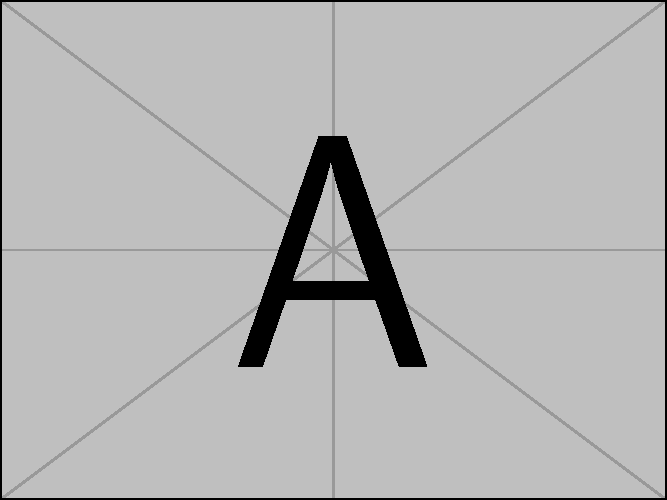
\includegraphics[width=0.23\textwidth]{example-image-a}
    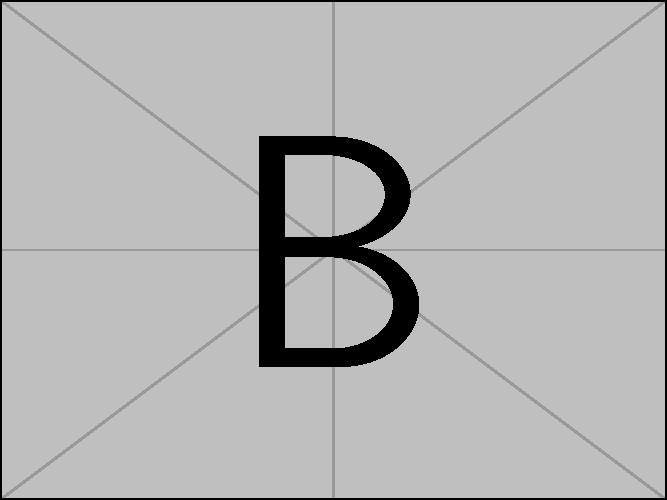
\includegraphics[width=0.23\textwidth]{example-image-b}
    \caption{A figure with two images placed side by side.} \label{fig:figure2}
\end{figure}
 % two images
\begin{figure}[thb] \centering
    \includegraphics[width=0.23\textwidth]{example-image}
    \includegraphics[width=0.23\textwidth]{example-image} 
    \\
    \includegraphics[width=0.23\textwidth]{example-image}
    \includegraphics[width=0.23\textwidth]{example-image} 
    \caption{A figure with four images.} \label{fig:figure3}
\end{figure}
 % four images
\begin{figure}[t] \centering
    \makebox[0.108\textwidth]{\scriptsize (a) Method 1}
    \makebox[0.108\textwidth]{\scriptsize (b) Method 2}
    \makebox[0.108\textwidth]{\scriptsize (c) Method 3}
    \makebox[0.108\textwidth]{\scriptsize (d) Method 4}
    \\
    \includegraphics[width=0.108\textwidth]{example-image}
    \includegraphics[width=0.108\textwidth]{example-image}
    \includegraphics[width=0.108\textwidth]{example-image}
    \includegraphics[width=0.108\textwidth]{example-image}
    \\
    \includegraphics[width=0.108\textwidth]{example-image}
    \includegraphics[width=0.108\textwidth]{example-image}
    \includegraphics[width=0.108\textwidth]{example-image}
    \includegraphics[width=0.108\textwidth]{example-image}
    \\
    \includegraphics[width=0.108\textwidth]{example-image}
    \includegraphics[width=0.108\textwidth]{example-image}
    \includegraphics[width=0.108\textwidth]{example-image}
    \includegraphics[width=0.108\textwidth]{example-image}
    \\
    \caption{A figure with text header.} 
    \label{fig:teaser}
\end{figure}
 % four images with text header
\begin{figure}[t] \centering
    \makebox[0.01\textwidth]{}
    \makebox[0.108\textwidth]{\scriptsize Input 1}
    \makebox[0.108\textwidth]{\scriptsize Input 2}
    \makebox[0.108\textwidth]{\scriptsize Input 3}
    \makebox[0.108\textwidth]{\scriptsize Input 4}
    \\
    \raisebox{0.1\height}{\makebox[0.01\textwidth]{\rotatebox{90}{\makecell{\scriptsize Method A}}}}
    \includegraphics[width=0.108\textwidth]{example-image}
    \includegraphics[width=0.108\textwidth]{example-image}
    \includegraphics[width=0.108\textwidth]{example-image}
    \includegraphics[width=0.108\textwidth]{example-image}
    \\
    \raisebox{0.1\height}{\makebox[0.01\textwidth]{\rotatebox{90}{\makecell{\scriptsize Method B}}}}
    \includegraphics[width=0.108\textwidth]{example-image}
    \includegraphics[width=0.108\textwidth]{example-image}
    \includegraphics[width=0.108\textwidth]{example-image}
    \includegraphics[width=0.108\textwidth]{example-image}
    \\
    \raisebox{0.1\height}{\makebox[0.01\textwidth]{\rotatebox{90}{\makecell{\scriptsize Method C}}}}
    \includegraphics[width=0.108\textwidth]{example-image}
    \includegraphics[width=0.108\textwidth]{example-image}
    \includegraphics[width=0.108\textwidth]{example-image}
    \includegraphics[width=0.108\textwidth]{example-image}
    \\
    \caption{A figure with vertical text for illustration.} 
    \label{fig:teaser}
\end{figure}

 % four images with vertical text
\begin{figure}[t] \centering
    \raisebox{1.5\height}{\makebox[0.055\textwidth]{\makecell{\small (a) \\ \footnotesize Version 1}}}
    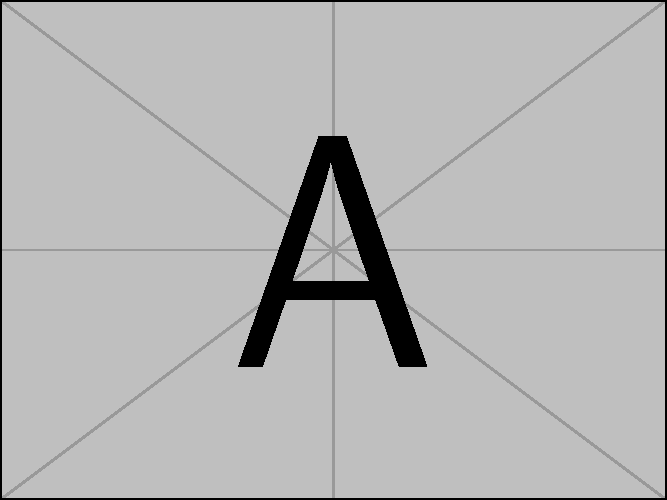
\includegraphics[width=0.175\textwidth]{example-image-a} \hfill
    \raisebox{1.5\height}{\makebox[0.055\textwidth]{\makecell{\small (b) \\ \footnotesize Version 2}}}
    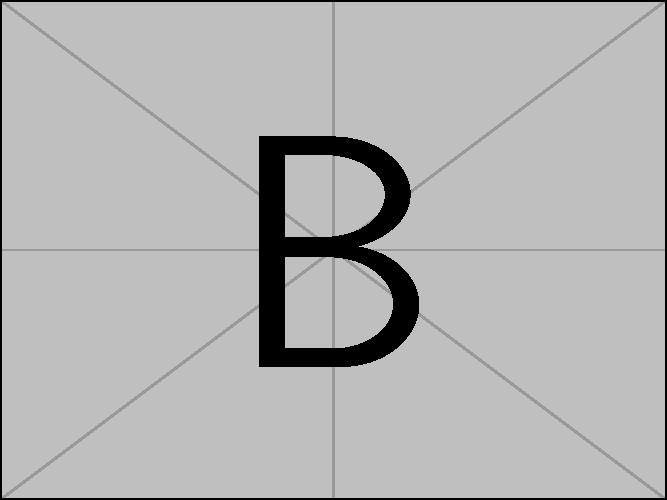
\includegraphics[width=0.175\textwidth]{example-image-b} 
    \\
    \caption{A figure with two sub-figures.} \label{fig:figure6}
\end{figure}

 % two sub figures
\begin{figure}[thbp]
    \centering
    \includegraphics[width=0.15\textwidth]{example-image}
    \includegraphics[width=0.15\textwidth]{example-image}
    \includegraphics[width=0.15\textwidth]{example-image}
    \\
    \makebox[0.48\textwidth]{\small (a) Figure A} 
    \\ \vspace{0.5em}
    \includegraphics[width=0.235\textwidth]{example-image}
    \includegraphics[width=0.235\textwidth]{example-image}
     \\
    \makebox[0.235\textwidth]{\small (b) Figure B}
    \makebox[0.235\textwidth]{\small (c) Figure C}
    \caption{A figure with three sub-figures.}
    \label{fig:fig15}
\end{figure}
 % figure numeric results and color bar

%\subsection{Examples for the Two-column Figures}

\begin{figure*}[thbp] \centering
    \includegraphics[width=\textwidth,height=0.4\textwidth]{example-image}
    \caption{A simple two-column figure.} \label{fig:figure7}
\end{figure*}
 % single image
\begin{figure*}[t] \centering
    \makebox[0.12\textwidth]{\footnotesize (a) Method 1}
    \makebox[0.12\textwidth]{\footnotesize (b) Method 2}
    \makebox[0.12\textwidth]{\footnotesize (c) Method 3}
    \makebox[0.12\textwidth]{\footnotesize (d) Method 4}
    \makebox[0.12\textwidth]{\footnotesize (e) Method 5}
    \makebox[0.12\textwidth]{\footnotesize (f) Method 6}
    \makebox[0.12\textwidth]{\footnotesize (g) Method 7}
    \makebox[0.12\textwidth]{\footnotesize (h) Method 8}
    \\
    \includegraphics[width=0.12\textwidth]{example-image}
    \includegraphics[width=0.12\textwidth]{example-image}
    \includegraphics[width=0.12\textwidth]{example-image}
    \includegraphics[width=0.12\textwidth]{example-image}
    \includegraphics[width=0.12\textwidth]{example-image}
    \includegraphics[width=0.12\textwidth]{example-image}
    \includegraphics[width=0.12\textwidth]{example-image}
    \includegraphics[width=0.12\textwidth]{example-image}
    \\
    \includegraphics[width=0.12\textwidth]{example-image}
    \includegraphics[width=0.12\textwidth]{example-image}
    \includegraphics[width=0.12\textwidth]{example-image}
    \includegraphics[width=0.12\textwidth]{example-image}
    \includegraphics[width=0.12\textwidth]{example-image}
    \includegraphics[width=0.12\textwidth]{example-image}
    \includegraphics[width=0.12\textwidth]{example-image}
    \includegraphics[width=0.12\textwidth]{example-image}
    \\
    \includegraphics[width=0.12\textwidth]{example-image}
    \includegraphics[width=0.12\textwidth]{example-image}
    \includegraphics[width=0.12\textwidth]{example-image}
    \includegraphics[width=0.12\textwidth]{example-image}
    \includegraphics[width=0.12\textwidth]{example-image}
    \includegraphics[width=0.12\textwidth]{example-image}
    \includegraphics[width=0.12\textwidth]{example-image}
    \includegraphics[width=0.12\textwidth]{example-image}
    \\
    \caption{A two-column figure with multiple images and text header.} 
    \label{fig:figure8}
\end{figure*}
 % multiple images
\newcommand{\largefigsize}{0.160}
\newcommand{\smallboxsize}{0.076}
\newcommand{\smallfigsize}{0.076}
\newcommand{\rheightsize}{0.77}
\newcommand{\vspacesize}{-2}
\newcommand{\hspacesize}{-3}

\begin{figure*}[t] \centering
    \makebox[0.24\textwidth]{\footnotesize (a) Input frame}
    \makebox[0.24\textwidth]{\footnotesize (b) Method A}
    \makebox[0.24\textwidth]{\footnotesize (c) Method B}
    \makebox[0.24\textwidth]{\footnotesize (d) Method C}
    \\
    \includegraphics[width=\largefigsize\textwidth]{example-image}\hspace{\hspacesize pt}
    \raisebox{\rheightsize\height}{
        \makebox[\smallboxsize\textwidth]{
            \makecell{
                \includegraphics[width=\smallfigsize\textwidth]{example-image}\\[\vspacesize pt]
                \includegraphics[width=\smallfigsize\textwidth]{example-image}
            }
        }
    }\hfill
    \includegraphics[width=\largefigsize\textwidth]{example-image}\hspace{\hspacesize pt}
    \raisebox{\rheightsize\height}{
        \makebox[\smallboxsize\textwidth]{
            \makecell{
                \includegraphics[width=\smallfigsize\textwidth]{example-image}\\[\vspacesize pt]
                \includegraphics[width=\smallfigsize\textwidth]{example-image}
            }
        }
    }\hfill
    \includegraphics[width=\largefigsize\textwidth]{example-image}\hspace{\hspacesize pt}
    \raisebox{\rheightsize\height}{
        \makebox[\smallboxsize\textwidth]{
            \makecell{
                \includegraphics[width=\smallfigsize\textwidth]{example-image}\\[\vspacesize pt]
                \includegraphics[width=\smallfigsize\textwidth]{example-image}
            }
        }
    }\hfill
    \includegraphics[width=\largefigsize\textwidth]{example-image}\hspace{\hspacesize pt}
    \raisebox{\rheightsize\height}{
        \makebox[\smallboxsize\textwidth]{
            \makecell{
                \includegraphics[width=\smallfigsize\textwidth]{example-image}\\[\vspacesize pt]
                \includegraphics[width=\smallfigsize\textwidth]{example-image}
            }
        }
    }
    \\
    \includegraphics[width=\largefigsize\textwidth]{example-image}\hspace{\hspacesize pt}
    \raisebox{\rheightsize\height}{
        \makebox[\smallboxsize\textwidth]{
            \makecell{
                \includegraphics[width=\smallfigsize\textwidth]{example-image}\\[\vspacesize pt]
                \includegraphics[width=\smallfigsize\textwidth]{example-image}
            }
        }
    }\hfill
    \includegraphics[width=\largefigsize\textwidth]{example-image}\hspace{\hspacesize pt}
    \raisebox{\rheightsize\height}{
        \makebox[\smallboxsize\textwidth]{
            \makecell{
                \includegraphics[width=\smallfigsize\textwidth]{example-image}\\[\vspacesize pt]
                \includegraphics[width=\smallfigsize\textwidth]{example-image}
            }
        }
    }\hfill
    \includegraphics[width=\largefigsize\textwidth]{example-image}\hspace{\hspacesize pt}
    \raisebox{\rheightsize\height}{
        \makebox[\smallboxsize\textwidth]{
            \makecell{
                \includegraphics[width=\smallfigsize\textwidth]{example-image}\\[\vspacesize pt]
                \includegraphics[width=\smallfigsize\textwidth]{example-image}
            }
        }
    }\hfill
    \includegraphics[width=\largefigsize\textwidth]{example-image}\hspace{\hspacesize pt}
    \raisebox{\rheightsize\height}{
        \makebox[\smallboxsize\textwidth]{
            \makecell{
                \includegraphics[width=\smallfigsize\textwidth]{example-image}\\[\vspacesize pt]
                \includegraphics[width=\smallfigsize\textwidth]{example-image}
            }
        }
    }
    \\
    \caption{A figure with multiple images, each with two zoom-in patches (horizontal).} 
    \label{fig:fig9}
\end{figure*}

 % multiple images with two zoom in patches (horizontal)
\begin{figure*}[t] \centering
    \newcommand{\hwidth}{1pt}
    \newcommand{\imgwidth}{0.24\textwidth}
    \newcommand{\patchwidth}{0.115\textwidth}
    \makebox[\imgwidth]{\small Overlapped Input}
    \makebox[\imgwidth]{\small Method A}
    \makebox[\imgwidth]{\small Method B} 
    \makebox[\imgwidth]{\small Method C} 
    \\
    \includegraphics[width=\imgwidth]{example-image}
    \includegraphics[width=\imgwidth]{example-image}
    \includegraphics[width=\imgwidth]{example-image}
    \includegraphics[width=\imgwidth]{example-image}
    \\[2pt]
    \makebox[\imgwidth]{%
        \includegraphics[width=\patchwidth]{example-image}\hspace{\hwidth}
        \includegraphics[width=\patchwidth]{example-image}} 
    \makebox[\imgwidth]{%
        \includegraphics[width=\patchwidth]{example-image}\hspace{\hwidth}
        \includegraphics[width=\patchwidth]{example-image}}
    \makebox[\imgwidth]{%
        \includegraphics[width=\patchwidth]{example-image}\hspace{\hwidth}
        \includegraphics[width=\patchwidth]{example-image}}
    \makebox[\imgwidth]{%
        \includegraphics[width=\patchwidth]{example-image}\hspace{\hwidth}
        \includegraphics[width=\patchwidth]{example-image}}
    \\[-0.1em]
    \makebox[\textwidth]{\small (a) Results on data A.} 
    \\[0.5em]
    \includegraphics[width=\imgwidth]{example-image}
    \includegraphics[width=\imgwidth]{example-image}
    \includegraphics[width=\imgwidth]{example-image}
    \includegraphics[width=\imgwidth]{example-image}
    \\[2pt]
    \makebox[\imgwidth]{%
        \includegraphics[width=\patchwidth]{example-image}\hspace{\hwidth}
        \includegraphics[width=\patchwidth]{example-image}} 
    \makebox[\imgwidth]{%
        \includegraphics[width=\patchwidth]{example-image}\hspace{\hwidth}
        \includegraphics[width=\patchwidth]{example-image}}
    \makebox[\imgwidth]{%
        \includegraphics[width=\patchwidth]{example-image}\hspace{\hwidth}
        \includegraphics[width=\patchwidth]{example-image}}
    \makebox[\imgwidth]{%
        \includegraphics[width=\patchwidth]{example-image}\hspace{\hwidth}
        \includegraphics[width=\patchwidth]{example-image}}
    \\[-0.1em]
    \makebox[\textwidth]{\small (a) Results on data B.} 
    \\[0.5em]
    \caption{A figure with two sub-figures. The sub-figure contains multiple images, each with two zoom-in patches (vertical).} 
    \label{fig:fig9}
\end{figure*}

 % multiple images with two zoom in patches (vertical) 
\begin{figure*}[thb] \centering
\begin{minipage}[t]{0.48\linewidth}
    \includegraphics[width=\textwidth,height=0.4\textwidth]{example-image}
    \caption{Two figures placed side by side. Figure A (left).} \label{tab:table10A}
\end{minipage}\hfill
\begin{minipage}[t]{0.48\linewidth}
    \includegraphics[width=\textwidth,height=0.4\textwidth]{example-image}
    \caption{Two figures placed side by side. Figure B (right).} \label{tab:table10B}
\end{minipage}
\end{figure*}
 % two figure placed side-by-side
\begin{figure*}[t]
\begin{minipage}[c]{0.49\textwidth} \centering
    \caption{A figure with caption at the right. This is useful for single-column paper (\eg, ECCV) to save space for narrow figures.} \label{fig:fig12}
\end{minipage}\hfill
\begin{minipage}[c]{0.48\textwidth}\centering
     \includegraphics[width=\textwidth,height=0.4\textwidth]{example-image} \\ \vspace{-0.4em}
\end{minipage}
\end{figure*}
 % figure with caption at the left
\begin{figure*}[t] \centering
    \begin{minipage}{0.96\textwidth}%
        \makebox[0.092\linewidth]{\scriptsize object} 
        \makebox[0.092\linewidth]{\scriptsize GT } 
        \makebox[0.092\linewidth]{\scriptsize Method A} 
        \makebox[0.092\linewidth]{\scriptsize Method B} 
        \makebox[0.092\linewidth]{\scriptsize Method C} 
        \hfill
        \makebox[0.092\linewidth]{\scriptsize object} 
        \makebox[0.092\linewidth]{\scriptsize GT } 
        \makebox[0.092\linewidth]{\scriptsize Method A} 
        \makebox[0.092\linewidth]{\scriptsize Method B} 
        \makebox[0.092\linewidth]{\scriptsize Method C} 
        \\
        \makebox[0.092\linewidth]{\includegraphics[width=0.092\linewidth]{example-image}}
        \makebox[0.092\linewidth]{\includegraphics[width=0.092\linewidth]{example-image}}
        \makebox[0.092\linewidth]{\includegraphics[width=0.092\linewidth]{example-image}}
        \makebox[0.092\linewidth]{\includegraphics[width=0.092\linewidth]{example-image}}
        \makebox[0.092\linewidth]{\includegraphics[width=0.092\linewidth]{example-image}} %
        \hfill
        \makebox[0.0920\linewidth]{\includegraphics[width=0.092\linewidth]{example-image}}
        \makebox[0.0920\linewidth]{\includegraphics[width=0.092\linewidth]{example-image}}
        \makebox[0.0920\linewidth]{\includegraphics[width=0.092\linewidth]{example-image}}
        \makebox[0.0920\linewidth]{\includegraphics[width=0.092\linewidth]{example-image}}
        \makebox[0.0920\linewidth]{\includegraphics[width=0.092\linewidth]{example-image}}
        \\
        \makebox[0.092\linewidth]{\scriptsize  (a) Data A} 
        \makebox[0.092\linewidth]{\scriptsize  } 
        \makebox[0.092\linewidth]{\scriptsize  \makecell{\scriptsize $1.41$ \\ \scriptsize$0.039$}} 
        \makebox[0.092\linewidth]{\scriptsize  \makecell{\scriptsize $5.44$ \\ \scriptsize$0.058$}} 
        \makebox[0.092\linewidth]{\scriptsize  \makecell{\scriptsize $2.43$ \\ \scriptsize$0.017$}} 
        \hfill
        \makebox[0.092\linewidth]{\scriptsize  (b) Data B} 
        \makebox[0.092\linewidth]{\scriptsize } 
        \makebox[0.0920\linewidth]{\scriptsize \makecell{\scriptsize$2.98 $ \\ \scriptsize$0.042$}} 
        \makebox[0.0920\linewidth]{\scriptsize \makecell{\scriptsize$10.36$ \\ \scriptsize$0.067$}} 
        \makebox[0.0920\linewidth]{\scriptsize \makecell{\scriptsize$33.22$ \\ \scriptsize$0.223$}} 
        \\
        \makebox[0.092\linewidth]{\includegraphics[width=0.092\linewidth]{example-image}}
        \makebox[0.092\linewidth]{\includegraphics[width=0.092\linewidth]{example-image}}
        \makebox[0.092\linewidth]{\includegraphics[width=0.092\linewidth]{example-image}}
        \makebox[0.092\linewidth]{\includegraphics[width=0.092\linewidth]{example-image}}
        \makebox[0.092\linewidth]{\includegraphics[width=0.092\linewidth]{example-image}} %
        \hfill
        \makebox[0.0920\linewidth]{\includegraphics[width=0.092\linewidth]{example-image}}
        \makebox[0.0920\linewidth]{\includegraphics[width=0.092\linewidth]{example-image}}
        \makebox[0.0920\linewidth]{\includegraphics[width=0.092\linewidth]{example-image}}
        \makebox[0.0920\linewidth]{\includegraphics[width=0.092\linewidth]{example-image}}
        \makebox[0.0920\linewidth]{\includegraphics[width=0.092\linewidth]{example-image}}
        \\
        \makebox[0.092\linewidth]{\scriptsize  (a) Data C} 
        \makebox[0.092\linewidth]{\scriptsize  } 
        \makebox[0.092\linewidth]{\scriptsize  \makecell{\scriptsize $1.41$ \\ \scriptsize$0.039$}} 
        \makebox[0.092\linewidth]{\scriptsize  \makecell{\scriptsize $5.44$ \\ \scriptsize$0.058$}} 
        \makebox[0.092\linewidth]{\scriptsize  \makecell{\scriptsize $2.43$ \\ \scriptsize$0.017$}} 
        \hfill
        \makebox[0.092\linewidth]{\scriptsize  (b) Data D} 
        \makebox[0.092\linewidth]{\scriptsize } 
        \makebox[0.0920\linewidth]{\scriptsize \makecell{\scriptsize$2.98 $ \\ \scriptsize$0.042$}} 
        \makebox[0.0920\linewidth]{\scriptsize \makecell{\scriptsize$10.36$ \\ \scriptsize$0.067$}} 
        \makebox[0.0920\linewidth]{\scriptsize \makecell{\scriptsize$33.22$ \\ \scriptsize$0.223$}} 
    \end{minipage}
    \begin{minipage}{0.01\textwidth} \centering
        \makebox[0.16\textwidth]{\scriptsize $0$} \\ \vspace{0.0em}
        \includegraphics[width=\linewidth,height=10\linewidth]{example-image} \\ \vspace{-0.6em}
        \makebox[0.16\textwidth]{\scriptsize $1$} \\
    \end{minipage}
    \caption{A figure with numerical results and color bar at the right.}
    \label{fig:fig14}
\end{figure*}
 % figure numeric results and color bar
\begin{figure*}[t] \centering
    \makebox[0.33\textwidth]{\footnotesize Input A}
    \makebox[0.33\textwidth]{\footnotesize Input B}
    \makebox[0.33\textwidth]{\footnotesize Input C}
    \\
    \includegraphics[width=0.33\textwidth]{example-image-a}
    \includegraphics[width=0.33\textwidth]{example-image-a}
    \includegraphics[width=0.33\textwidth]{example-image-a}
    \\
    \makebox[0.495\textwidth]{\footnotesize Overlapped Input} \hfill
    \makebox[0.495\textwidth]{\footnotesize Our Result}
    \\
    \includegraphics[width=0.495\textwidth]{example-image-b} \hfill
    \includegraphics[width=0.495\textwidth]{example-image-b}
    \\
    \makebox[0.162\textwidth]{\footnotesize Method A}
    \makebox[0.162\textwidth]{\footnotesize Method B}
    \makebox[0.162\textwidth]{\footnotesize Method C}
    \makebox[0.162\textwidth]{\footnotesize Method D}
    \makebox[0.162\textwidth]{\footnotesize Method E}
    \makebox[0.162\textwidth]{\footnotesize Method F}
    \\
    \includegraphics[width=0.162\textwidth]{example-image-c}
    \includegraphics[width=0.162\textwidth]{example-image-c}
    \includegraphics[width=0.162\textwidth]{example-image-c}
    \includegraphics[width=0.162\textwidth]{example-image-c}
    \includegraphics[width=0.162\textwidth]{example-image-c}
    \includegraphics[width=0.162\textwidth]{example-image-c}
    \\
    \includegraphics[width=0.162\textwidth]{example-image-c}
    \includegraphics[width=0.162\textwidth]{example-image-c}
    \includegraphics[width=0.162\textwidth]{example-image-c}
    \includegraphics[width=0.162\textwidth]{example-image-c}
    \includegraphics[width=0.162\textwidth]{example-image-c}
    \includegraphics[width=0.162\textwidth]{example-image-c}
    \\
    \caption{A figure with multi-level images.} 
    \label{fig:fig10}
\end{figure*}
 % multiple images organized with multi-level

\input{figures/mvps}

%\clearpage
%%%%%%%%% REFERENCES
%{\small
%\bibliographystyle{ieee_fullname}
%\bibliography{egbib}
%}

\end{document}
